\documentclass[crop,tikz]{standalone}

\usepackage{amsmath}

\tikzset {
  potato style/.style = {
    thick,
    fill=black!5,
    opacity=0.9,
    draw=black
  },
  pics/potato/.style args = {#1 #2 #3}{
    code = {
      \path ({-1.1*#1*(1+#3)}, {-1.1*#1*#2*(1+#3)}) rectangle ({1.1*#1*(1+#3)}, {1.1*#1*#2*(1+#3)});
      \filldraw[potato style, pic actions] plot [domain=0:360, samples=50]
      ({(1+0.5*#3*sin(2*\x+20))*(1+#3*sin(\x))*(1.0*#1*cos(\x))},
       {(1+0.5*#3*sin(2*\x+20))*(1+#3*sin(\x))*( #2*#1*sin(\x))})
       --cycle;
    }
  }
}

\begin{document}

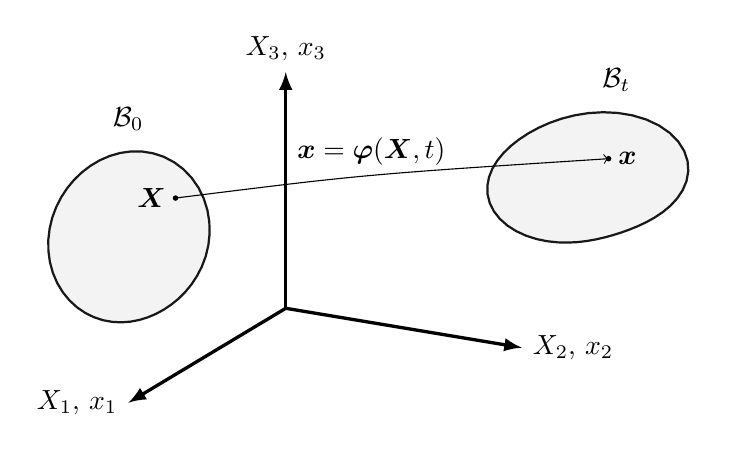
\begin{tikzpicture}[scale=1.0]

% --- Axes ---
\draw[-latex,very thick] (0,0) -- ( 0, 3.0) node[above] {$X_3,\,x_3$};
\draw[-latex,very thick] (0,0) -- ( 3,-0.5) node[right] {$X_2,\,x_2$};
\draw[-latex,very thick] (0,0) -- (-2,-1.2) node[left] {$X_1,\,x_1$};


% --- Reference configuration B_0 ---
\begin{scope}[shift={(-2,0.8)}]

  % Geometry
  \pic[thick] {potato=1.0 1.1 0.1};
  \node at (0,1.6) {$\mathcal{B}_0$};

  % Material point in B_0
  \coordinate (XR) at (0.6,0.6);
  \fill (XR) circle (1pt);
  \node[anchor=east] at (XR) {$\boldsymbol{X}$};

  % % Small area element in B_0
  % \draw (0.3,0.0) rectangle (0.6,0.3);

\end{scope}


% --- Current configuration B_t ---
\begin{scope}[shift={(3.8,1.5)}]

  % Geometry
  \pic[thick] {potato=1.2 0.7 0.2};
  \node at (0.4,1.4) {$\mathcal{B}_t$};

  % Spatial point in B_t
  \coordinate (xt) at (0.3,0.4);
  \fill (xt) circle (1pt);
  \node[anchor=west] at (xt) {$\boldsymbol{x}$};

  % % Small area element in B_t
  % \draw (1.1,-0.4) rectangle (1.4,-0.1);
\end{scope}


% --- Mapping arrow ---
\draw[->] (XR) .. controls (1,1.7) .. (xt)
    node[midway, above] {$\boldsymbol{x}=\boldsymbol{\varphi}(\boldsymbol{X},t)$};

% % --- Differential mappings ---
% \draw[->] (-2.55,0.35) .. controls (0,-0.5) .. (3.65,-0.05)
%     node[midway, below, align=left] {
%       $\mathrm{d}\boldsymbol{x}=\boldsymbol{F}\,\mathrm{d}\boldsymbol{X}$ \\
%       $\mathrm{d}a=\boldsymbol{H}\,\mathrm{d}A$ \\
%       $\mathrm{d}v=J\,\mathrm{d}V$
%       };

\end{tikzpicture}


\end{document}
